\section{Darstellung der Ergebnisse}
In diesem Kapitel werden die in der Methode erarbeiteten Erkennungsalgorithmen veranschaulicht. Hierzu gehören das ohne \textit{Transfer-Learning} entwickelte \textit{CNN} aus Kapitel \ref{cha:met:adjcnn}, das mittels GoogLeNet verbesserte \textit{CNN} (\textit{Transfer-Learning}) aus Kapitel \ref{cha:met:tl} sowie die finale Version mit \textit{Transfer-Learning} und Zusatzinformationen aus Kapitel \ref{cha:met:einfimpl}.

\subsection{CNN ohne \textit{Transfer-Learning}}
Dieses \textit{CNN} wurde von Grund auf neu konfiguriert und mit den künstlich erweiterten Trainingsdaten trainiert. Es besteht insgesamt aus 16 \textit{Layers} und mehr als 140'000 lernbaren \textit{Parametern} (siehe Kapitel \ref{cha:theo:neurons}) und besteht hauptsächlich aus drei \textit{Convolution}-\textit{Pooling}-Einheiten mit je einem \textit{ReLU-} und \textit{Normalization}-\textit{Layer}. Durch die Justierung einiger \textit{Meta-Parameter} konnte dieses \textit{CNN}s weiter auf die Pilzartenerkennung angepasst werden (\textit{Meta-Parameter} zum Aufbau und Training in Tabellen \ref{table:final_cnn_structure} und \ref{table:final_cnn_training} auf Seite \pageref{table:final_cnn_structure} f.).

Folgende Bestimmungsgenauigkeiten konnten durch dieses justierte \textit{CNN} erreicht werden:

\begin{table}[h]
	\begin{center}
		\def\arraystretch{1.4}
		\begin{tabular}{ c c c }
			Leistung mit Trainingsdaten &\qquad\qquad\qquad& Leistung mit Validierungsdaten \\
			89.4\% && \textbf{76.0\%}\footnotemark \\
		\end{tabular}
	\end{center}
\end{table}

\footnotetext{\label{fn:result_evaluation}Leistung gemittelt über 10 Testreihen, da durch grenzwertige Trainingsexemplare mit \textit{Data-Augmentation} verschiedene Resultate erzielt werden können. Um trotzdem ein zuverlässiges Resultat zu erhalten, wurden alle Validierungsdaten je 10 Mal eingespeist.}

Um einen besseren Einblick in die Zusammensetzung der Fehlerquote zu erhalten, dient die in Abbildung \ref{img:conf_mat_cnn} dargestellte Vertauschungsmatrix, bei der alle 560 Validierungsdaten je zehnmal vom \textit{CNN} bestimmt und entsprechend eingetragen worden sind.

Zwar ist die genaue Funktionsweise eines trainierten \textit{KNN}s wenn überhaupt nur schwierig nachzuvollziehen, jedoch lässt sich der erste Stritt der Informationsfilterung noch veranschaulichen. In Abbildung \ref{img:feature_maps_cnn} sind die Gewichtungen der 40 \textit{Feature-Maps} des ersten \textit{Convolution-Layers} abgebildet. Diese zeigen, auf welche Strukturen und Muster die jeweilige \textit{Feature-Map} anspricht.

\begin{figure}[h]
	\centering
	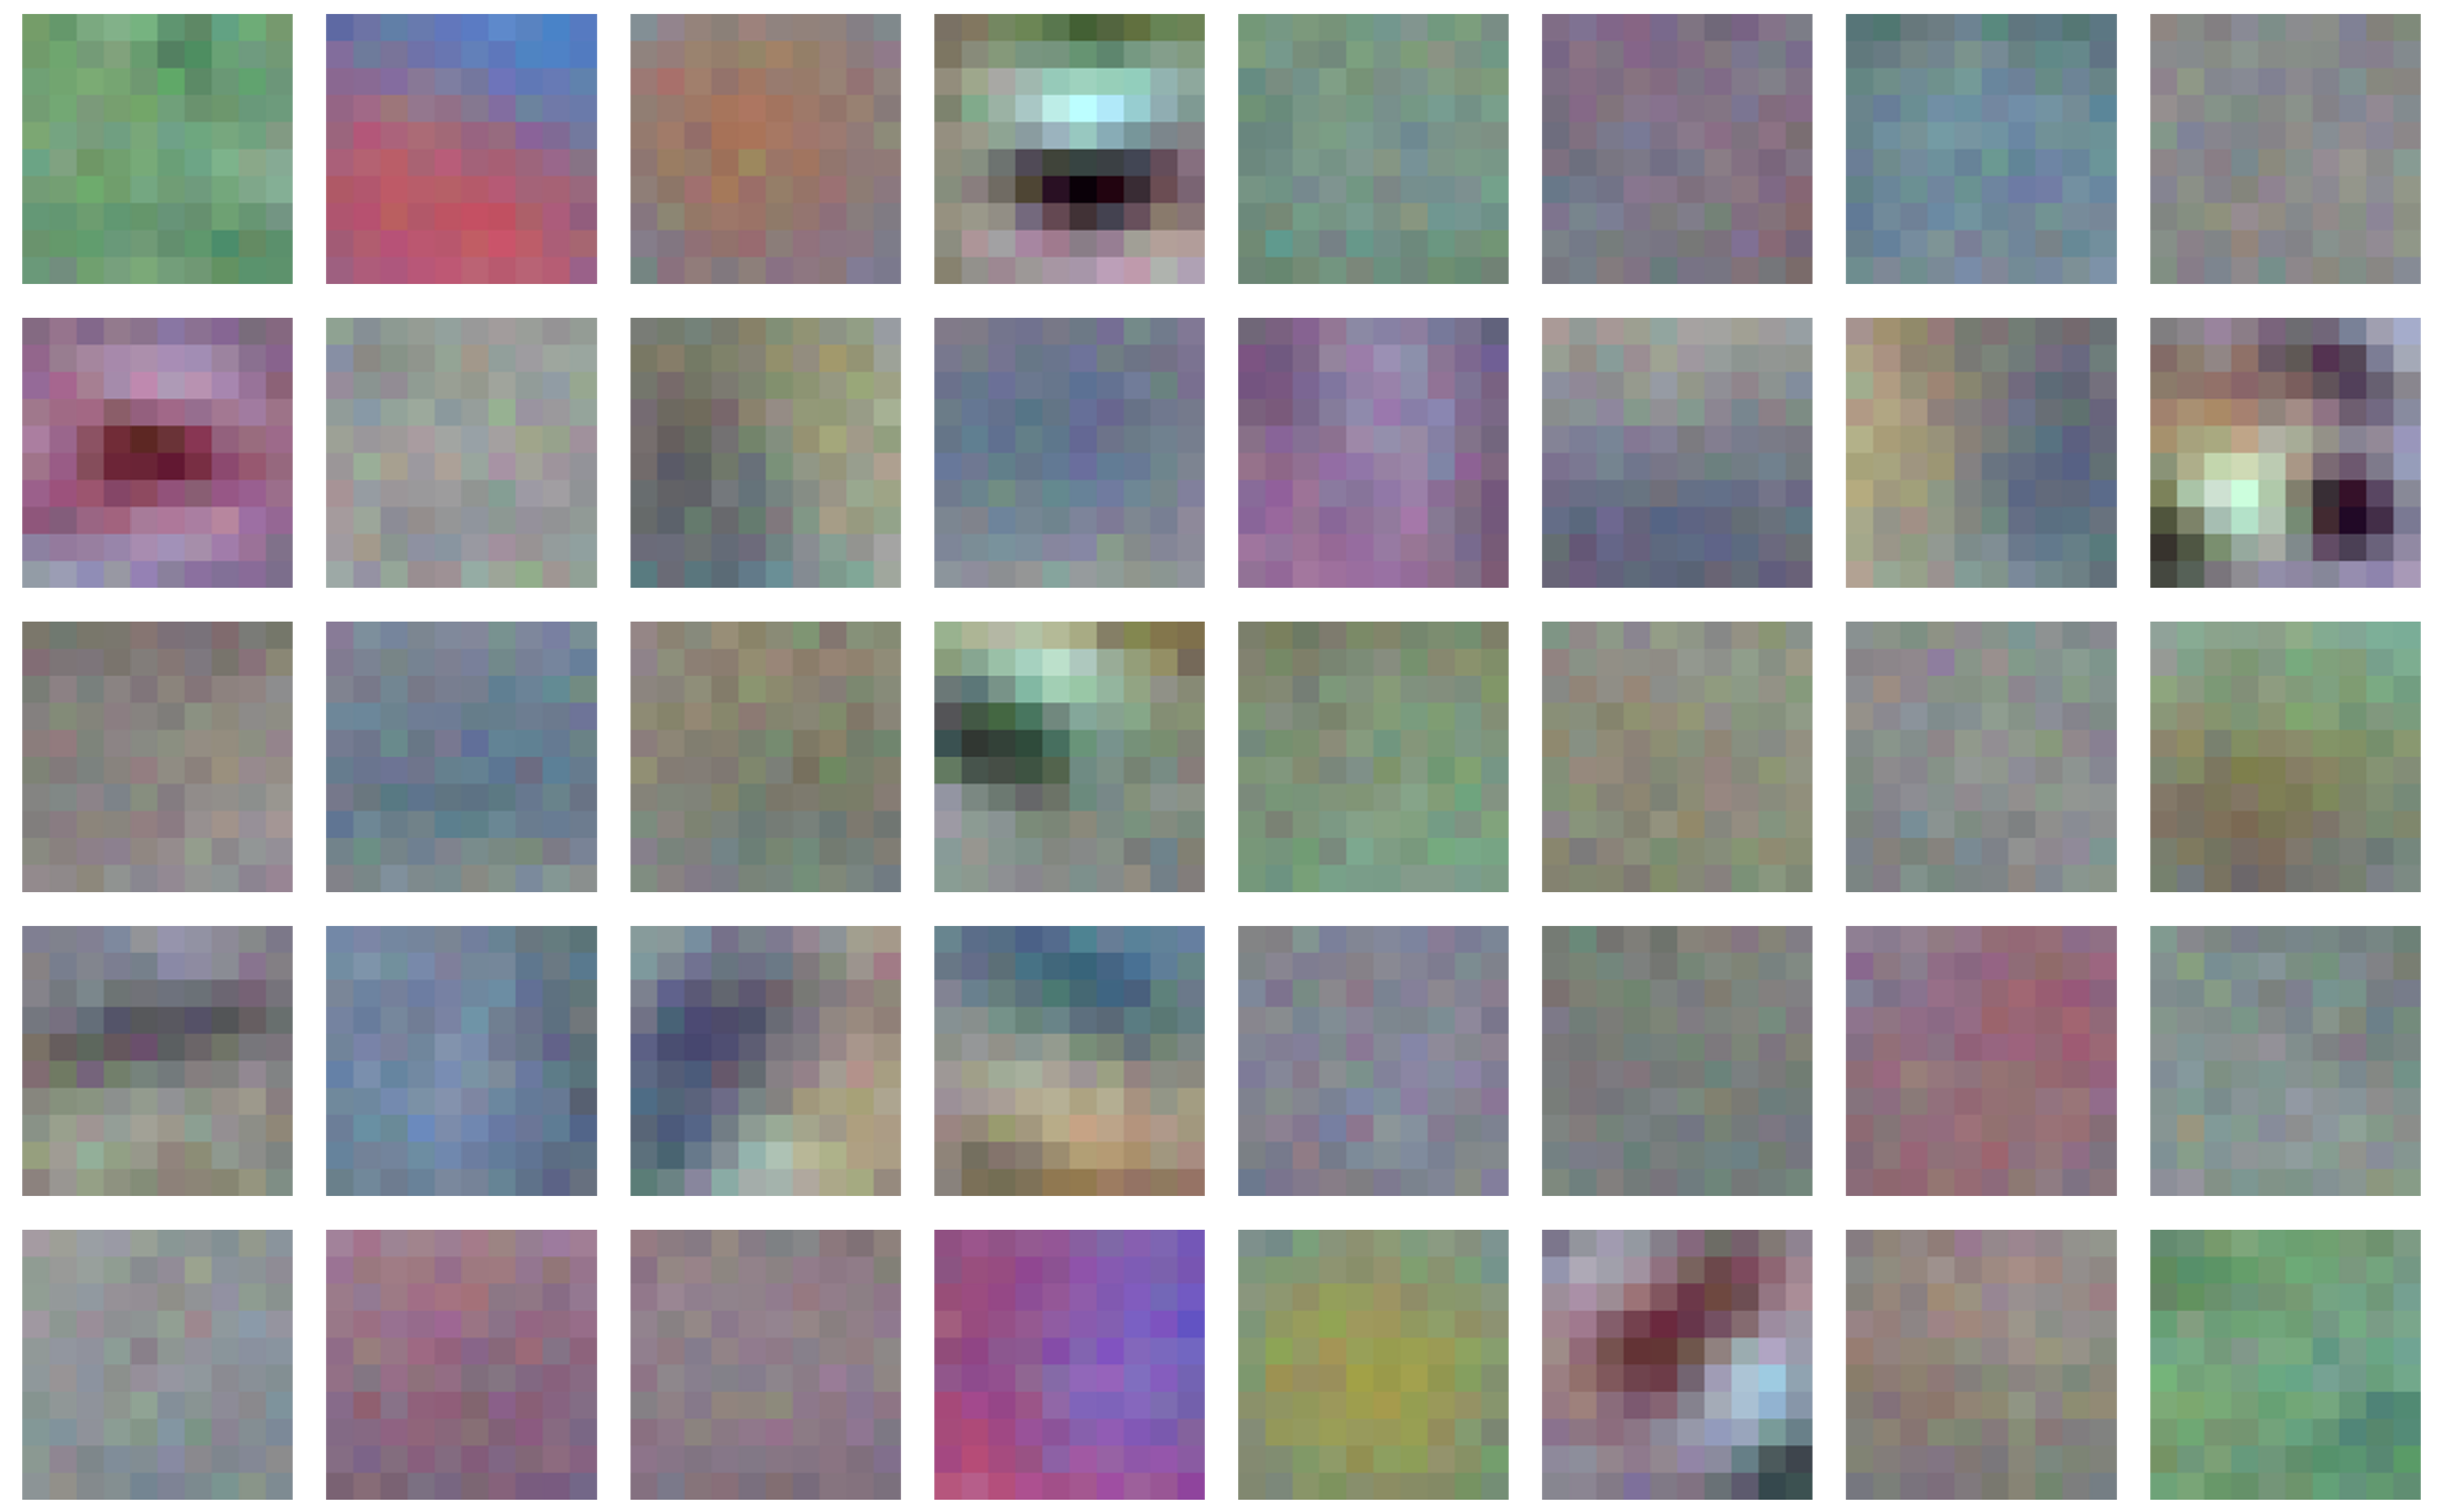
\includegraphics[width=0.8\textwidth]{feature_maps_cnn}
	\caption[\textit{Feature-Maps} vom justierten \textit{CNN}]{40 10$\times$10px \textit{Feature-Maps} vom erstem \textit{Convolution-Layer} des justierten \textit{CNN}s}
	\label{img:feature_maps_cnn}
\end{figure}
\begin{sidewaysfigure}
	\centering
	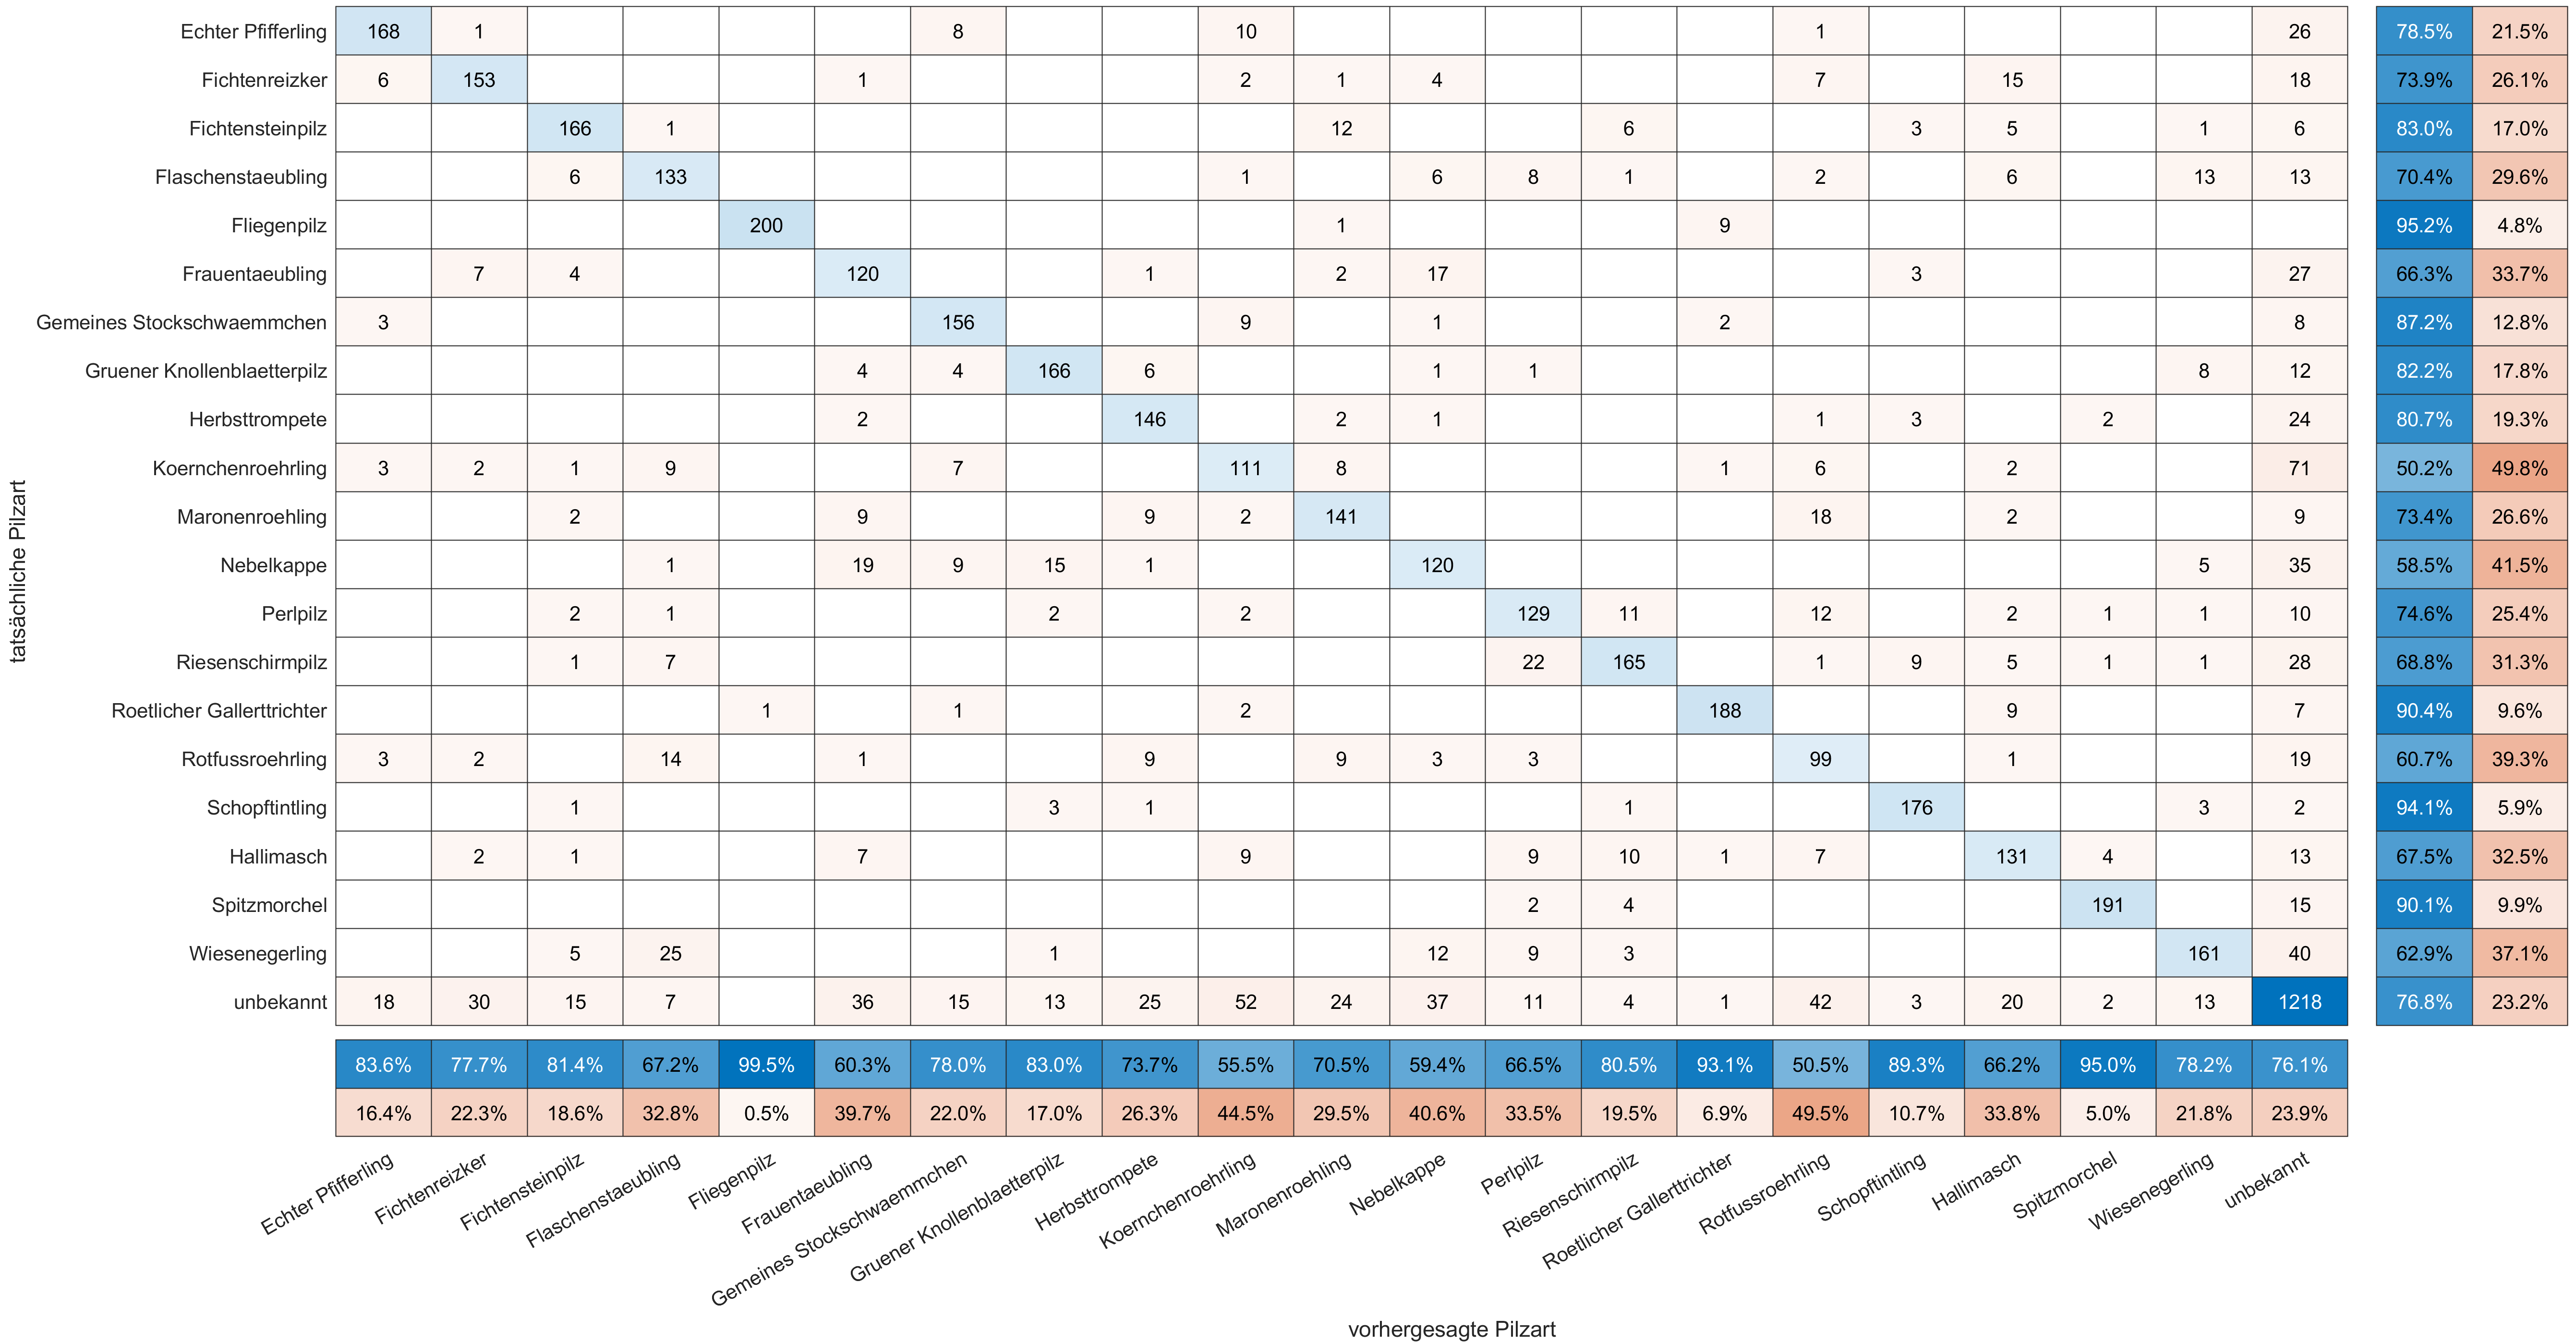
\includegraphics[width=\textwidth]{conf_mat_cnn}
	\caption[Vertauschungsmatrix des justierten \textit{CNN}s]{Vertauschungsmatrix des justierten \textit{CNN}s, Validierungsdaten je zehn mal bestimmt: Auf der Diagonalen befinden sich die Anzahl korrekt klassifizierten Validierungsdaten, die restlichen sind falsch bestimmt worden.}
	\label{img:conf_mat_cnn}
\end{sidewaysfigure}


\subsection{CNN mit \textit{Transfer-Learning}}
Als Ausgangslage dient GoogLeNet\cite{googlenet}, welches mittels \textit{Transfer-Learning} auf die Pilzerkennung umtrainiert worden ist. Hierzu wurde vor dem Training der letzte \textit{Fully-Connected-Layer} durch einen auf die Anzahl der Kategorien angepasster \textit{Fully-Connected-Layer} ersetzt und mit zufälligen Werten initialisiert. GoogLeNet verwendet neben konventionellen \textit{Convolution-Layers} auch sog. \textit{Inception-Module} (detaillierter Aufbau siehe \cite{googlenet}), durch welche die ausserordentliche Leistung von GoogLeNet erreicht werden kann. Mit insgesamt 9 solcher \textit{Inception-Module} weist das \textit{Transfer-CNN} eine totale Tiefe von 27 \textit{Layers} auf und enthält etwa 5.8 Millionen lernbare \textit{Parameter}. Beim Training wurde mittels verschiedenen Lernraten bewerkstelligt, dass die \textit{Parameter} des neuen \textit{Fully-Connected-Layers} (ca. 21'000) viel schneller angepasst werden als die der transferierten \textit{Layers}. Trainiert wurde das \textit{Transfer-CNN} ebenfalls mit Bildnormalisierung und \textit{Data-Augmentation} (alle \textit{Meta-Parameter} zum Aufbau und Training siehe Tabelle \ref{table:transfer_training} auf Seite \pageref{table:transfer_training}).

folgende Ergebnisse erzielt werden:

\begin{table}[h]
	\begin{center}
		\def\arraystretch{1.4}
		\begin{tabular}{ c c c }
			Leistung mit Trainingsdaten &\qquad\qquad\qquad& Leistung mit Validierungsdaten \\
			85.9\% && \textbf{84.8\%}\footnotemark
		\end{tabular}
	\end{center}
\end{table}

\footnotetext{Auch hier wurde das Ergebnis über 10 Testreihen gemittelt, siehe Fussnote \ref{fn:result_evaluation}}

Auch für das \textit{Transfer-CNN} ist in Abbildung \ref{img:conf_mat_transfer} zur Analyse der Fehlerquote die entsprechende Vertauschungsmatrix abgebildet, wobei die Validierungsdaten wiederum je zehn Mal bestimmt worden sind.

Für den Vergleich des \textit{Transfer-CNN}s mit dem justierten \textit{CNN} aus vorherigem Abschnitt werden zudem wieder die \textit{Feature-Maps} des ersten \textit{Convolution-Layers} in folgender Abbildung aufgezeigt.

\begin{figure}[h]
	\centering
	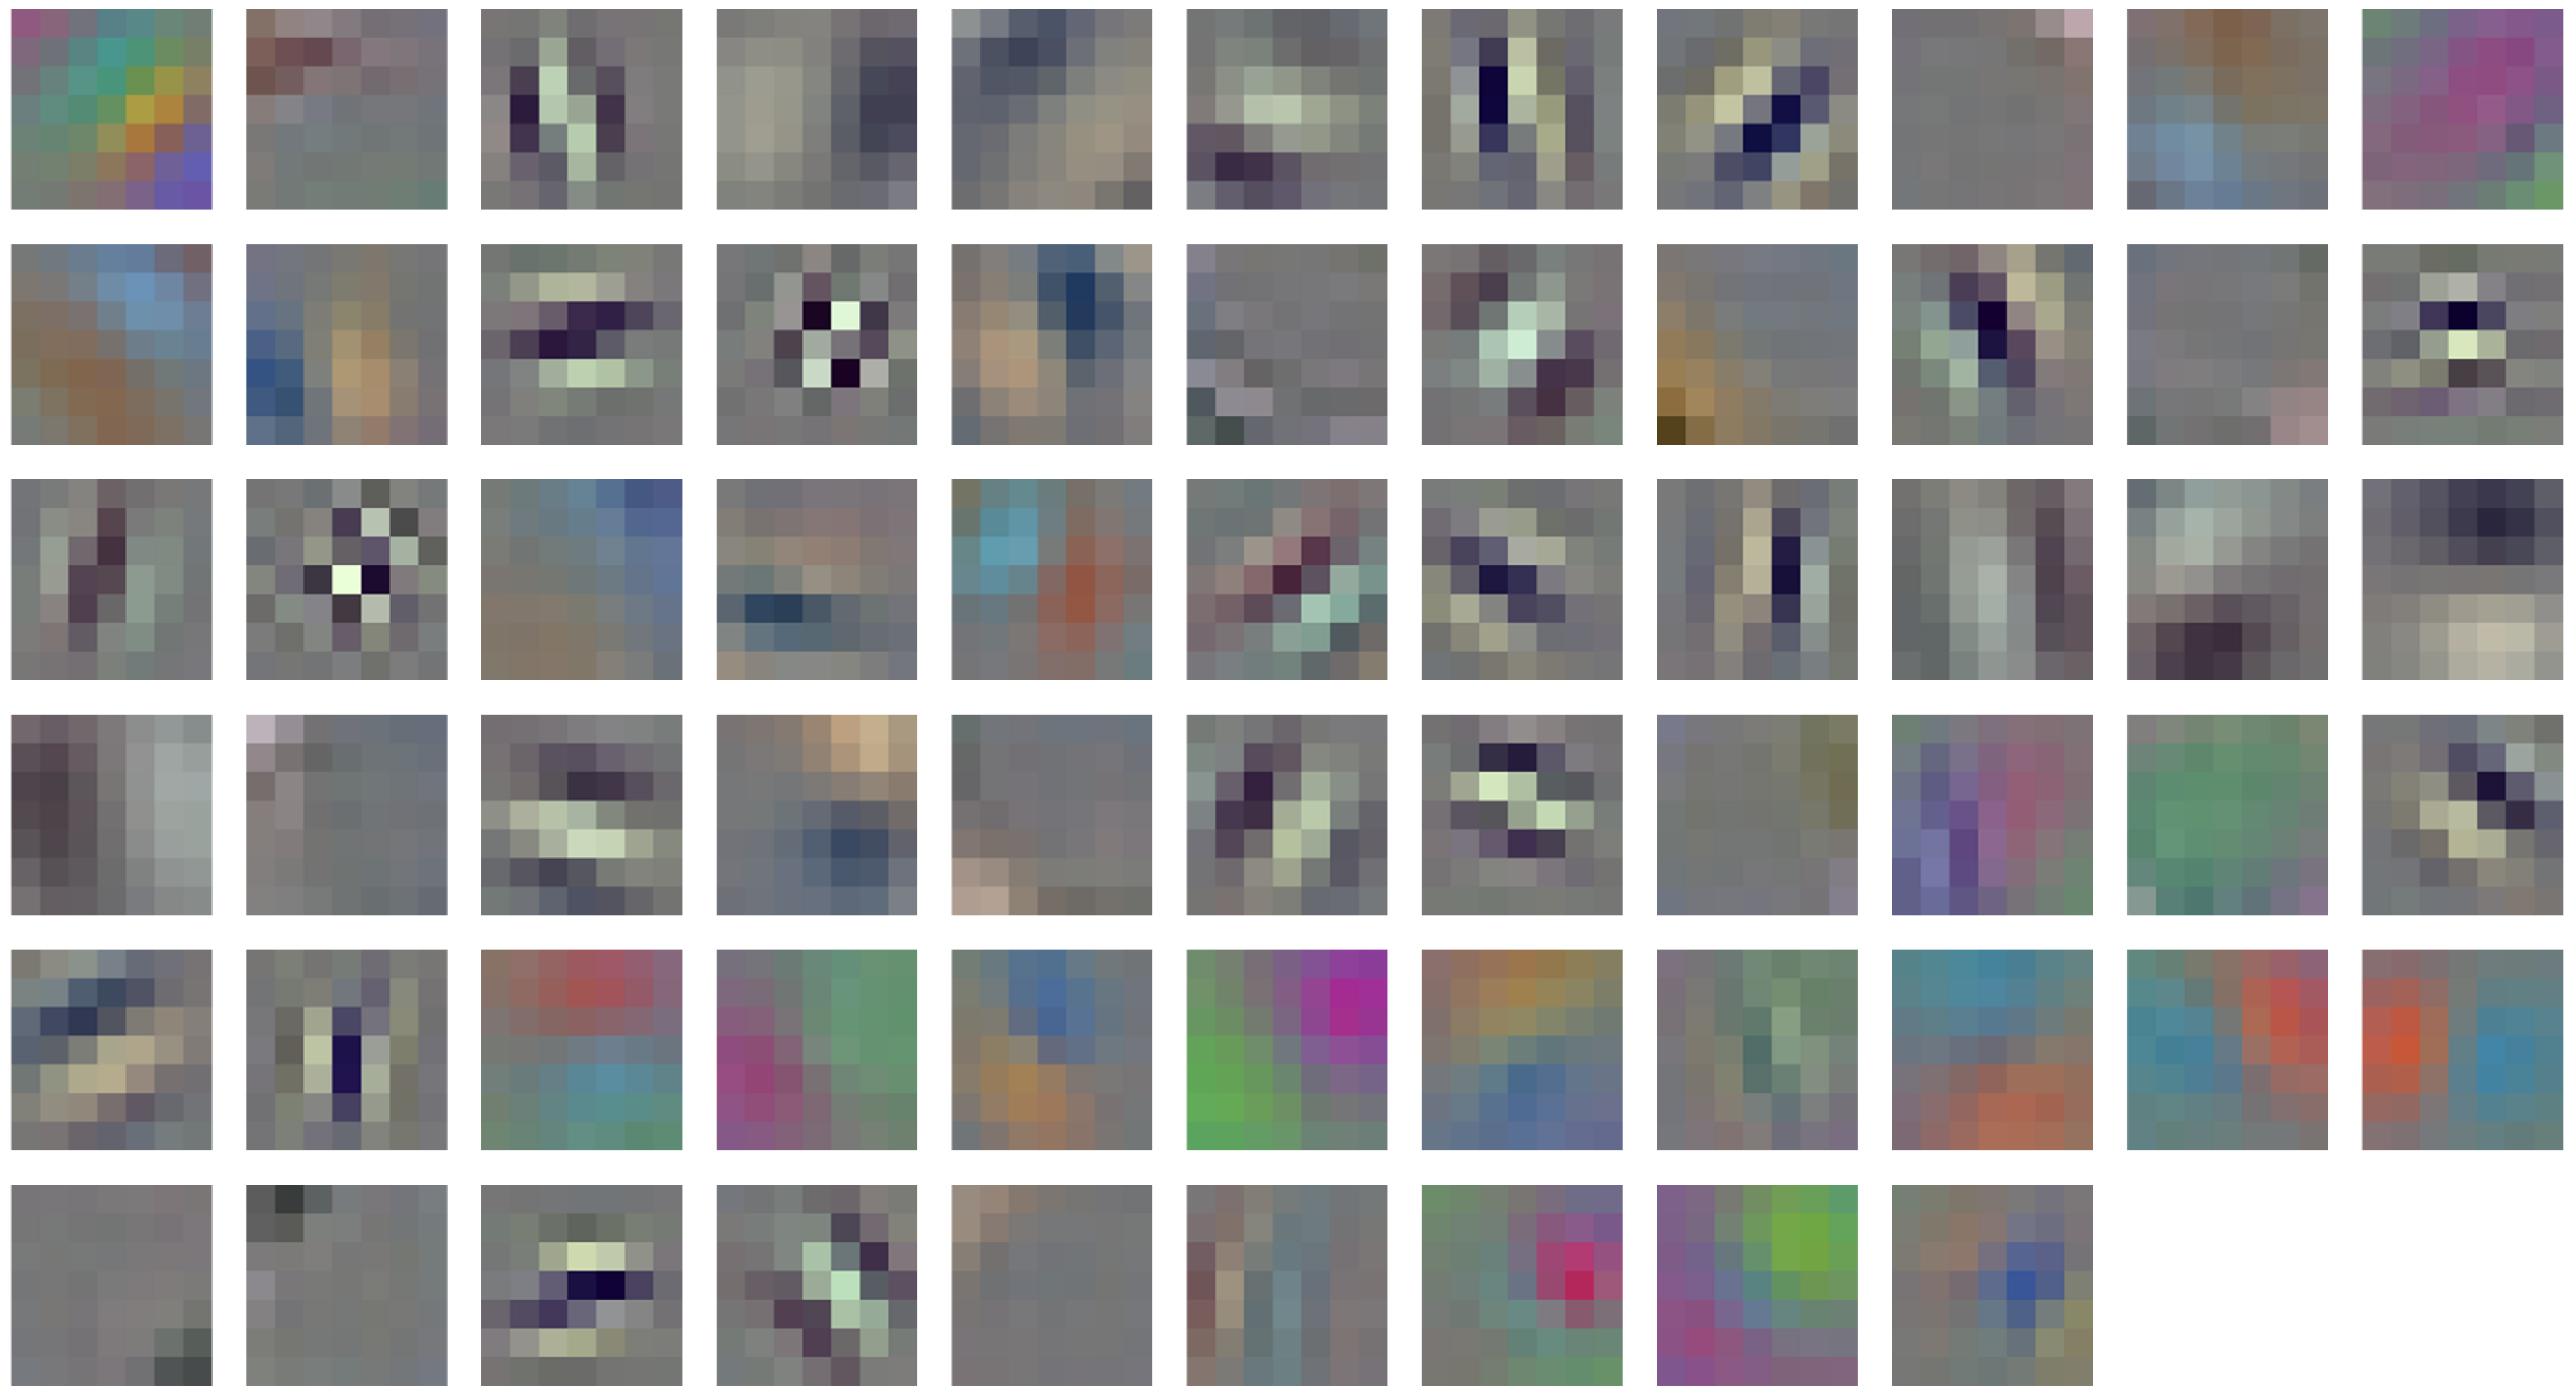
\includegraphics[width=\textwidth]{feature_maps_google_3}
	\caption[\textit{Feature-Maps} vom \textit{Transfer-CNN}]{64 7$\times$7px \textit{Feature-Maps} vom ersten \textit{Convolution-Layers} des \textit{Transfer-CNN}s}
	\label{img:feature_maps_transfer}
\end{figure}

\begin{sidewaysfigure}
	\centering
	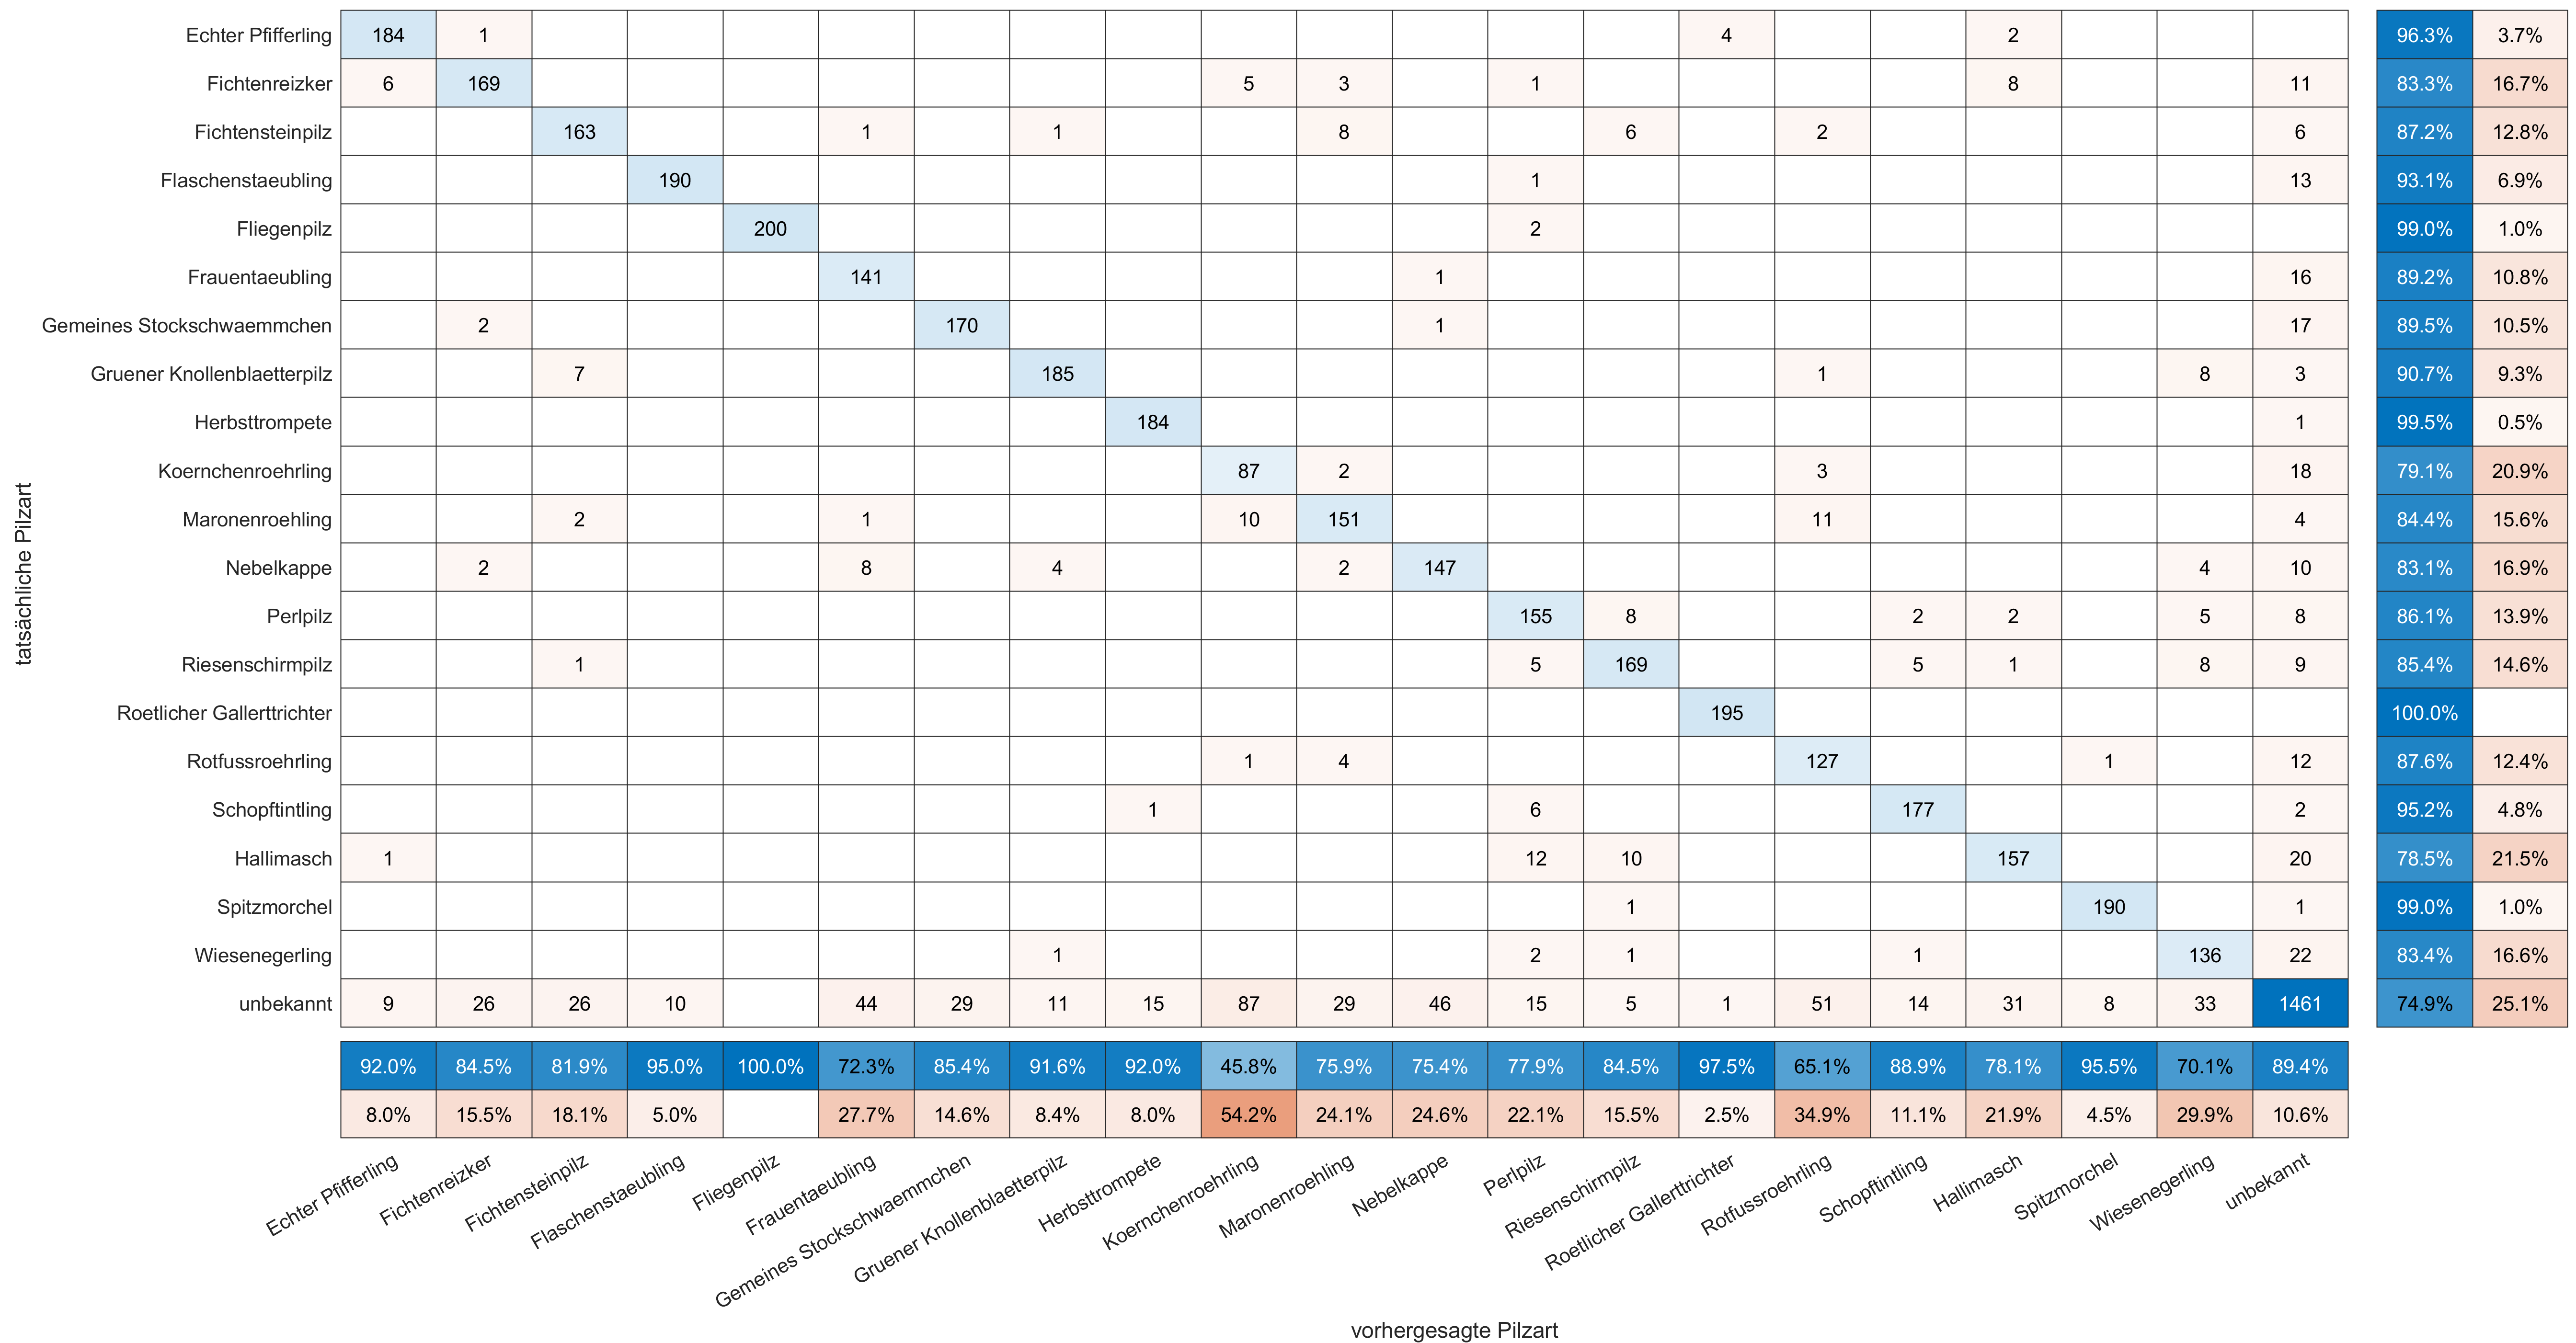
\includegraphics[width=\textwidth]{conf_mat_transfer}
	\caption[Vertauschungsmatrix des transferierten \textit{CNN}s]{Vertauschungsmatrix des \textit{Transfer-CNN}s, Validierungsdaten je zehn mal bestimmt: Auf der Diagonalen befinden sich die Anzahl korrekt klassifizierten Validierungsdaten, die restlichen sind falsch bestimmt worden.}
	\label{img:conf_mat_transfer}
\end{sidewaysfigure}

\newpage

\subsection{CNN mit \textit{Transfer-Learning} und Zusatzinformationen}

\begin{table}[h]
	\begin{center}
		\def\arraystretch{1.4}
		\begin{tabular}{ c c c c c}
			Leistung mit Trainingsdaten &\qquad\qquad\qquad& \multicolumn{3}{c}{Leistung mit Validierungsdaten} \\
			{\footnotesize \textit{50\% keine, 40\% teilweise, 10\% alle Inf.}}& &{\footnotesize  \textit{keine Inf.}} & {\footnotesize \textit{50\% der Inf.}} &{\footnotesize  \textit{alle Inf.}}\\
			91.5\% &								   & \textbf{88.0\%} & \textbf{95.4\% }& \textbf{98.5\%} \\
		\end{tabular}
	\end{center}
\end{table}
Blablablablablabla blablablabla blablablabla blablablabla blablablabla blablablabla blablablabla blablablabla blablablabla blablablabla blablablabla blablablabla blablablabla blablablabla blablablabla blablablabla blablablabla blablablabla blablablabla blablablabla blablablabla blablablabla blablablabla blablablabla


\begin{sidewaysfigure}
	\centering
	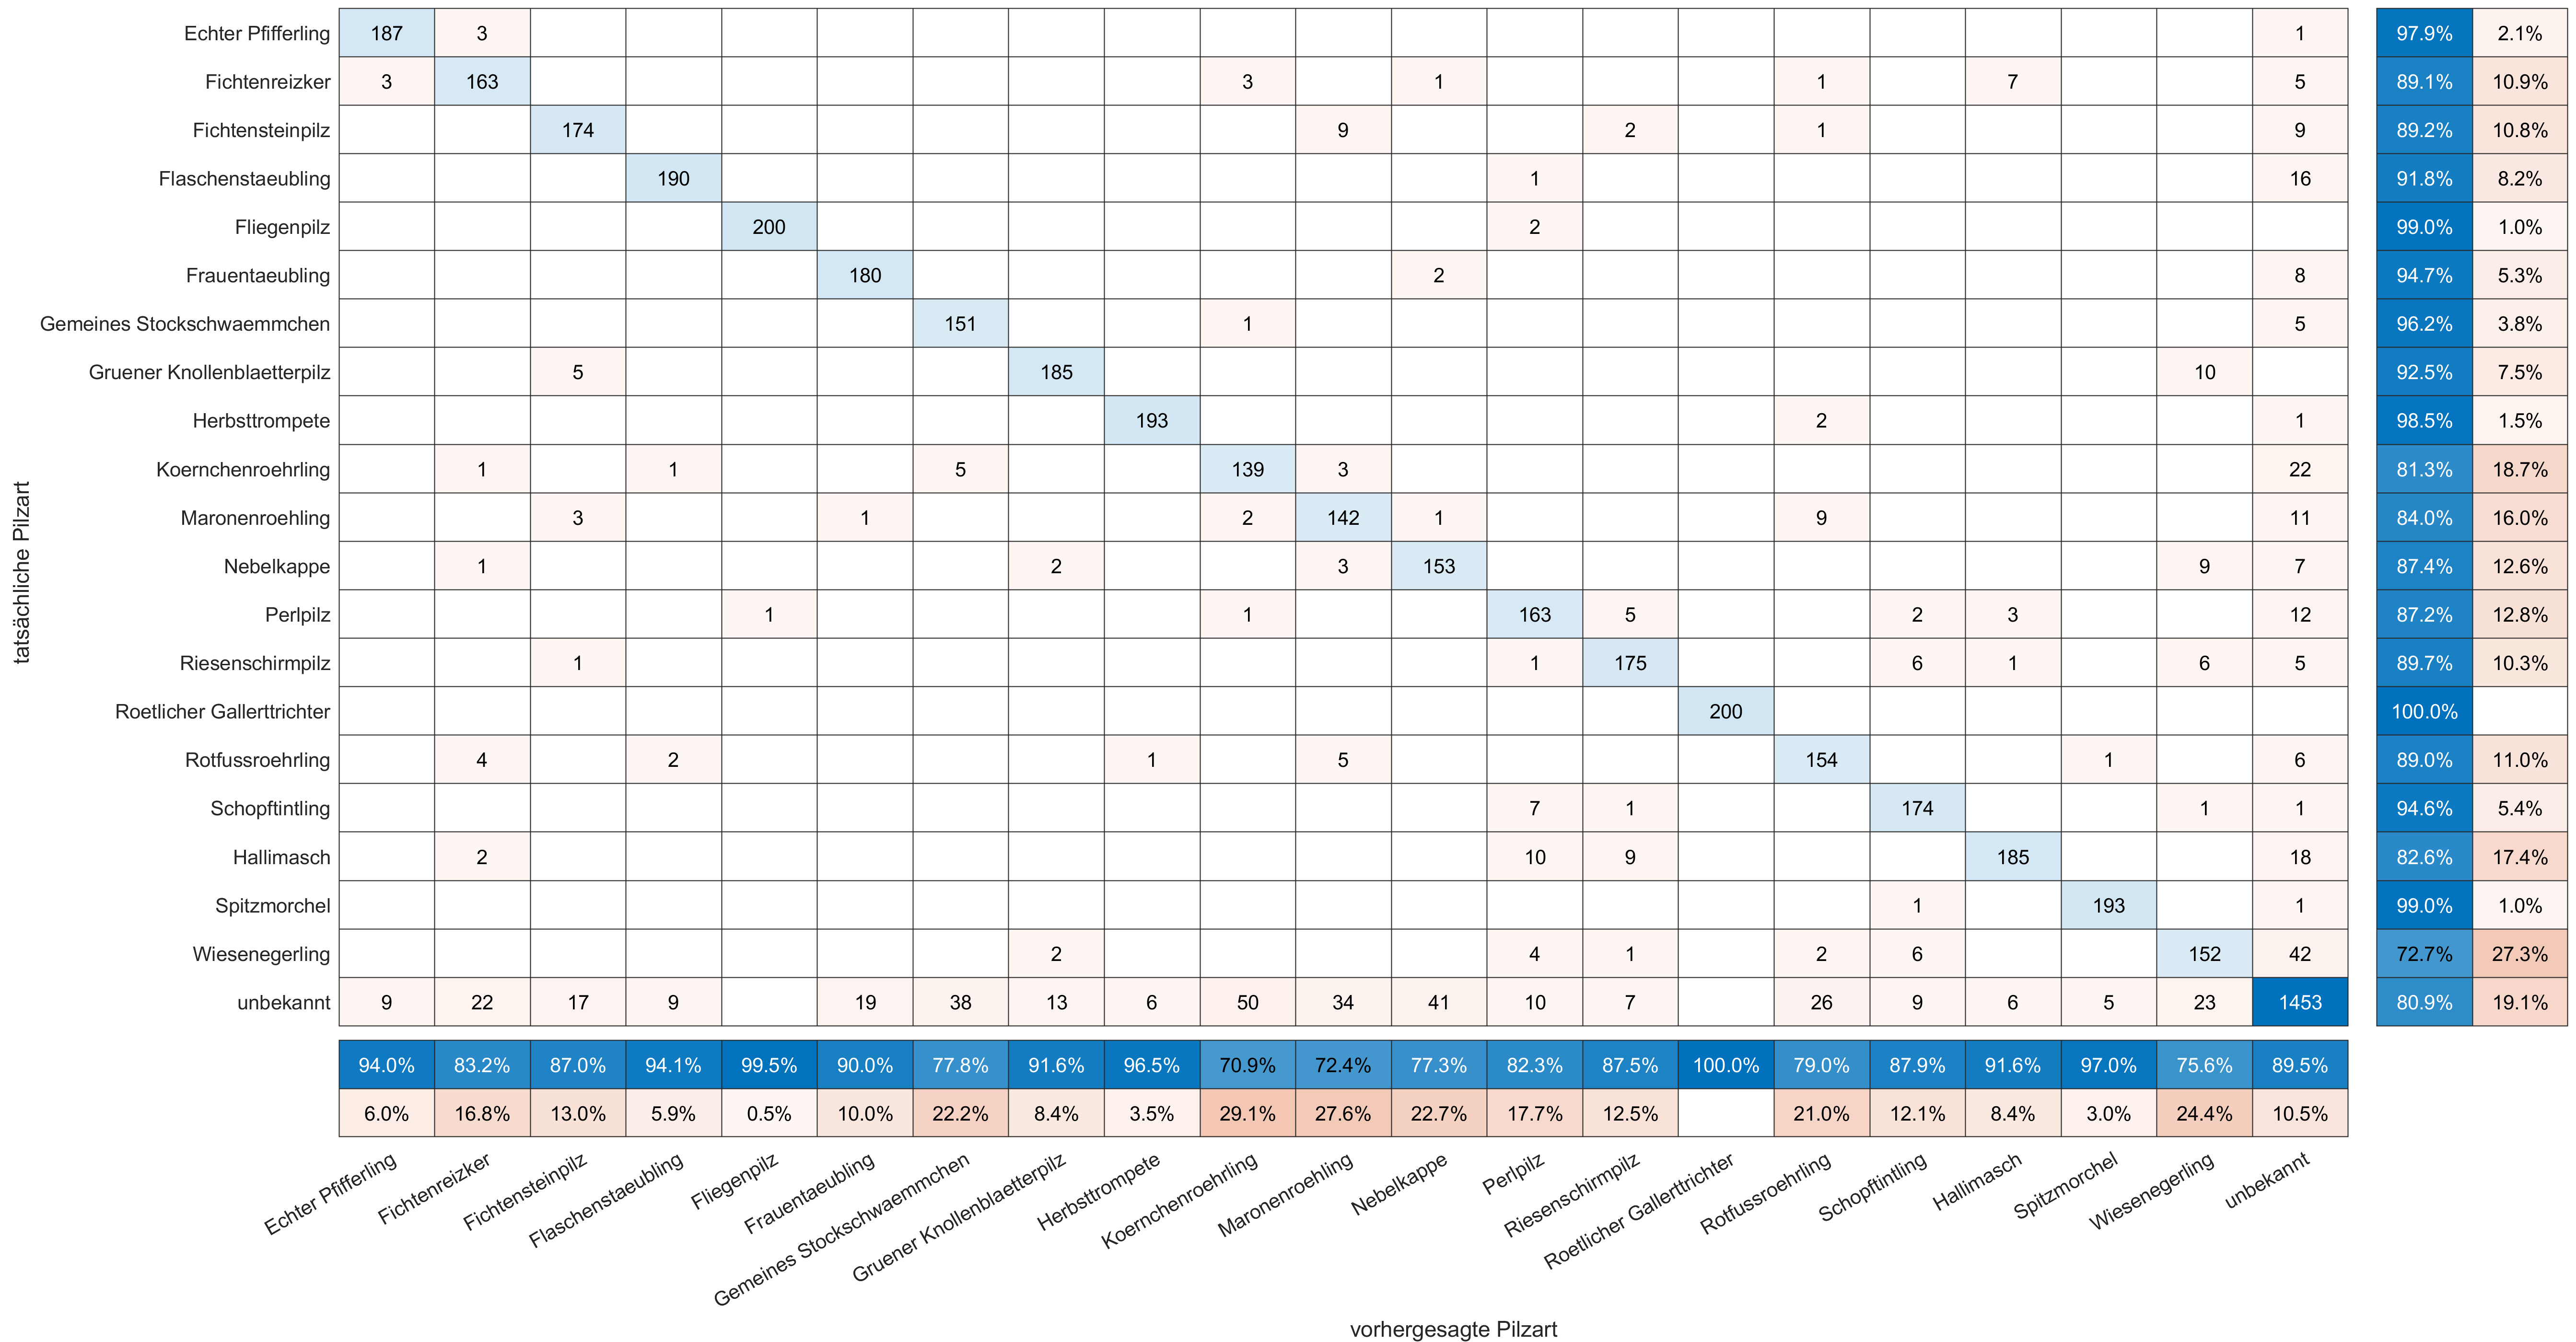
\includegraphics[width=\textwidth]{conf_mat_extra_none}
	\caption[Vertauschungsmatrix des Zusatzinformationen-\textit{Transfer-CNN}s ohne Zusatzinformationen]{Vertauschungsmatrix des Zusatzinformationen-\textit{Transfer-CNN}s, Bestimmung ohne Zusatzinformationen durchgeführt, Validierungsdaten je zehn mal bestimmt: Auf der Diagonalen befinden sich die Anzahl korrekt klassifizierten Validierungsdaten, die restlichen sind falsch bestimmt worden.}
	\label{img:conf_mat_extra_none}
\end{sidewaysfigure}


\begin{sidewaysfigure}
\centering
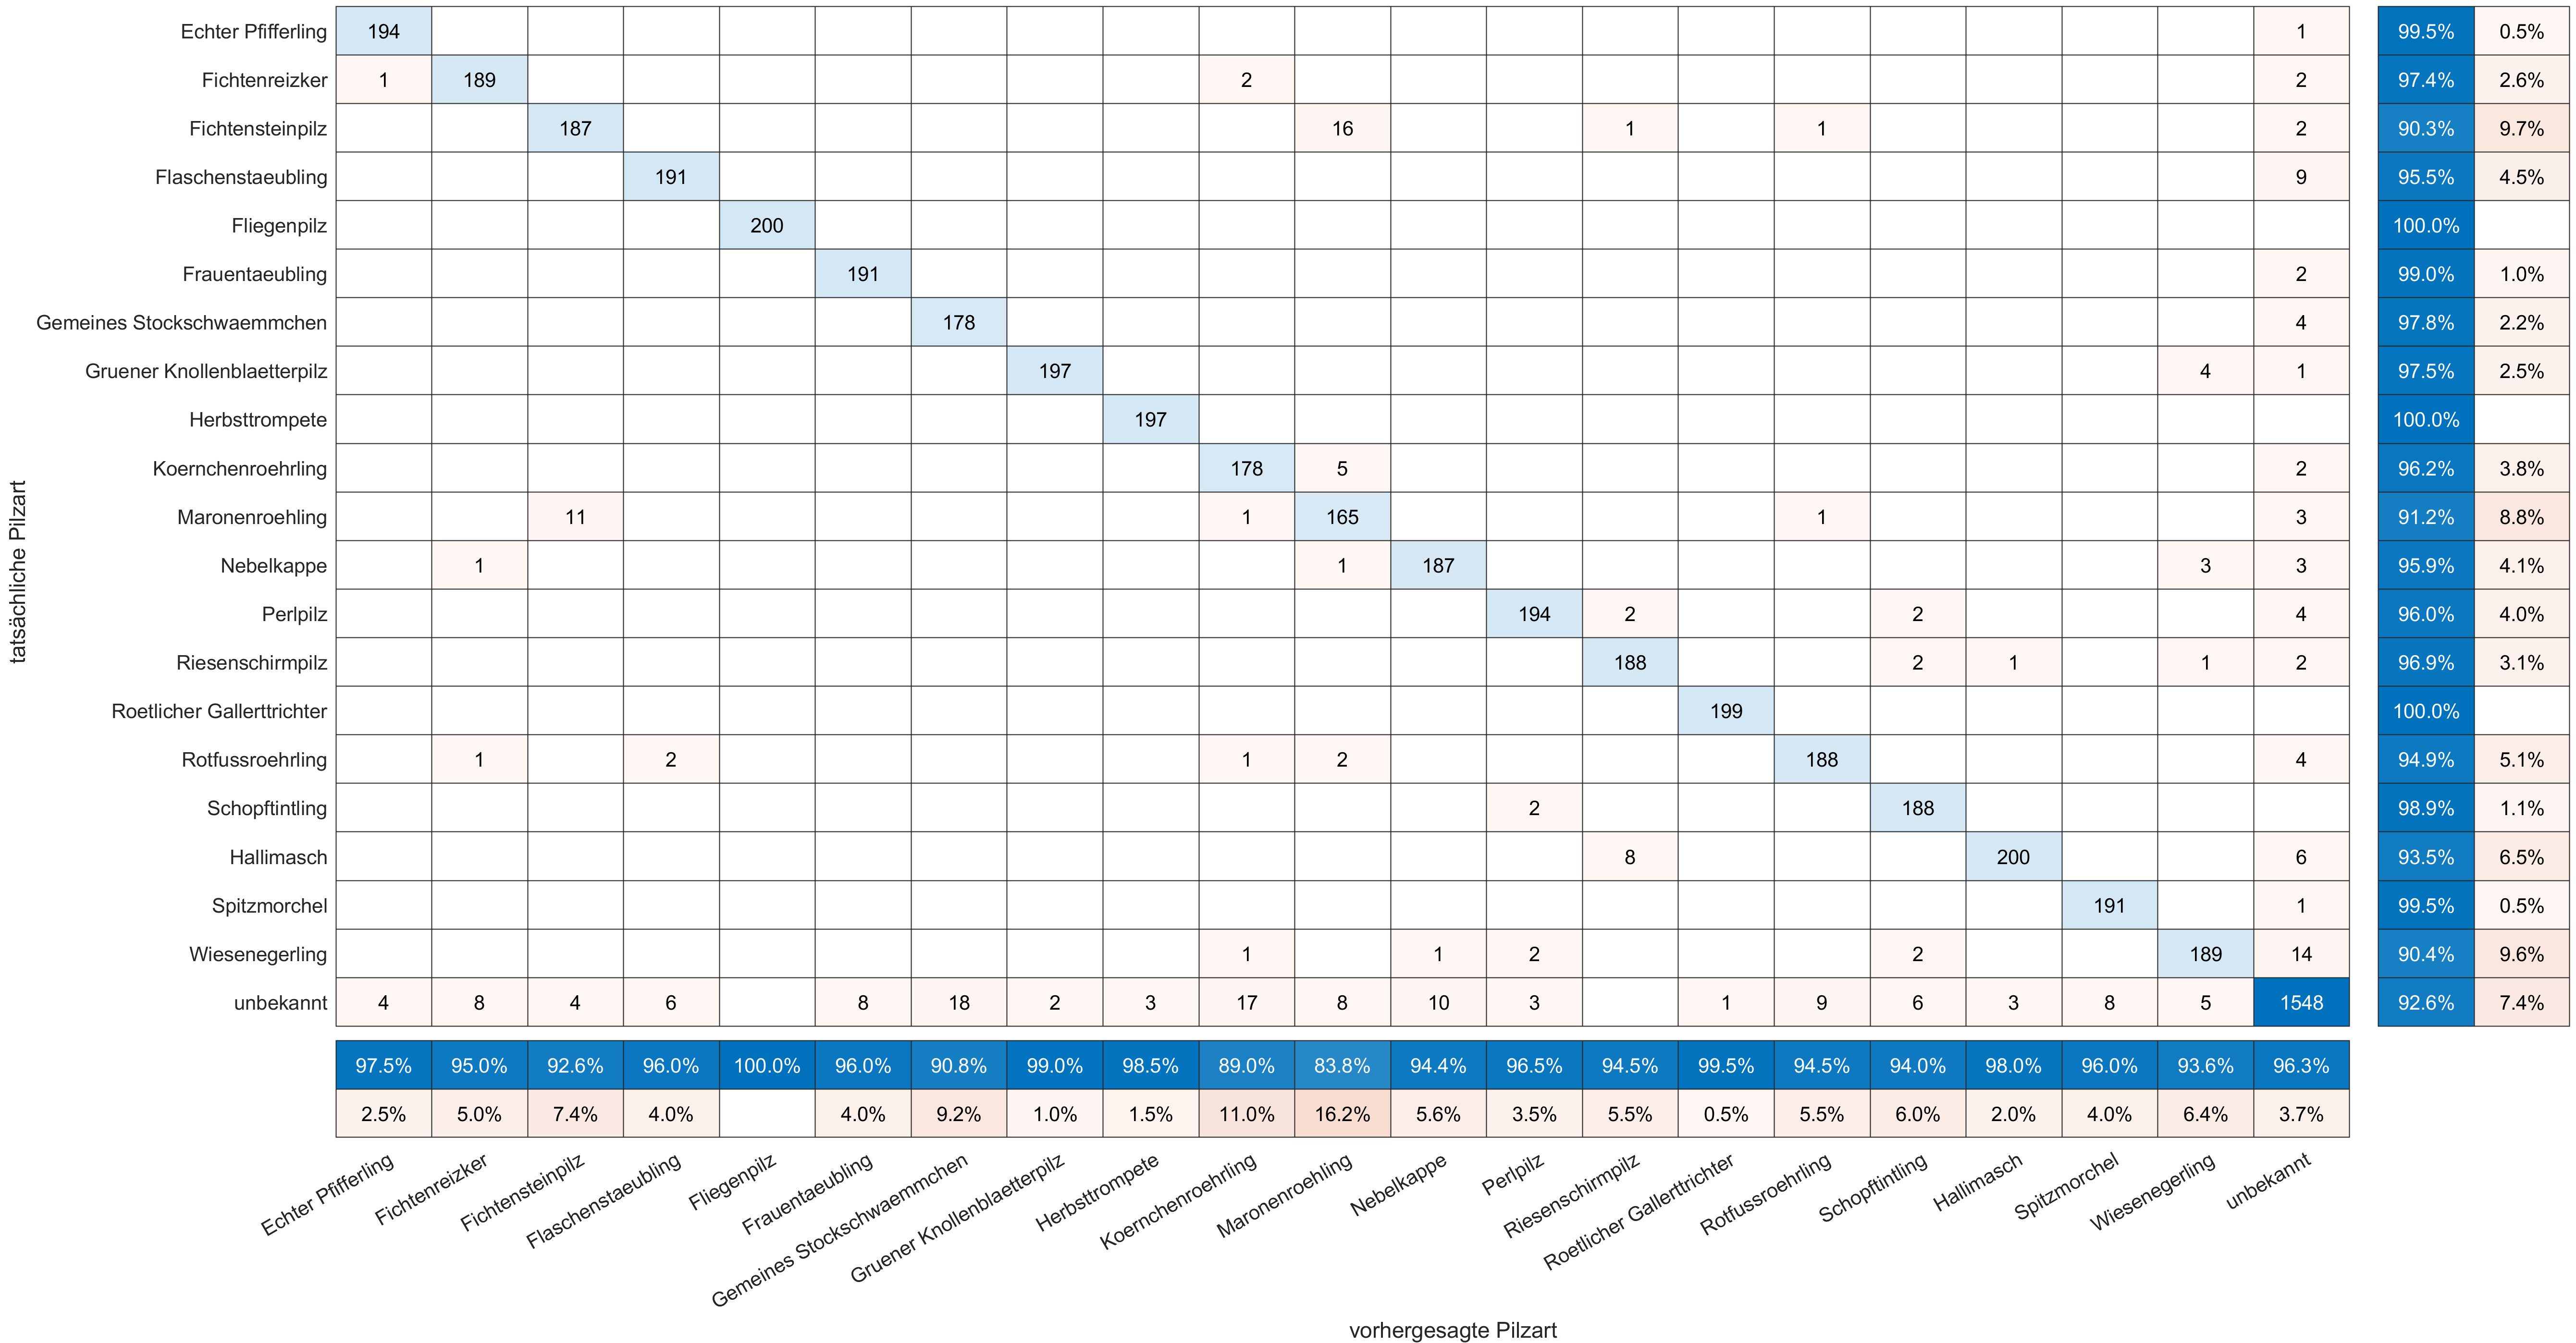
\includegraphics[width=\textwidth]{conf_mat_extra_half}
\caption[Vertauschungsmatrix des Zusatzinformationen-\textit{Transfer-CNN}s mit 50\% der Zusatzinformationen]{Vertauschungsmatrix des Zusatzinformationen-\textit{Transfer-CNN}s, für Bestimmung 50\% der Zusatzinformationen gegeben, Validierungsdaten je zehn mal bestimmt: Auf der Diagonalen befinden sich die Anzahl korrekt klassifizierten Validierungsdaten, die restlichen sind falsch bestimmt worden.}
\label{img:conf_mat_extra_half}
\end{sidewaysfigure}


\begin{sidewaysfigure}
\centering
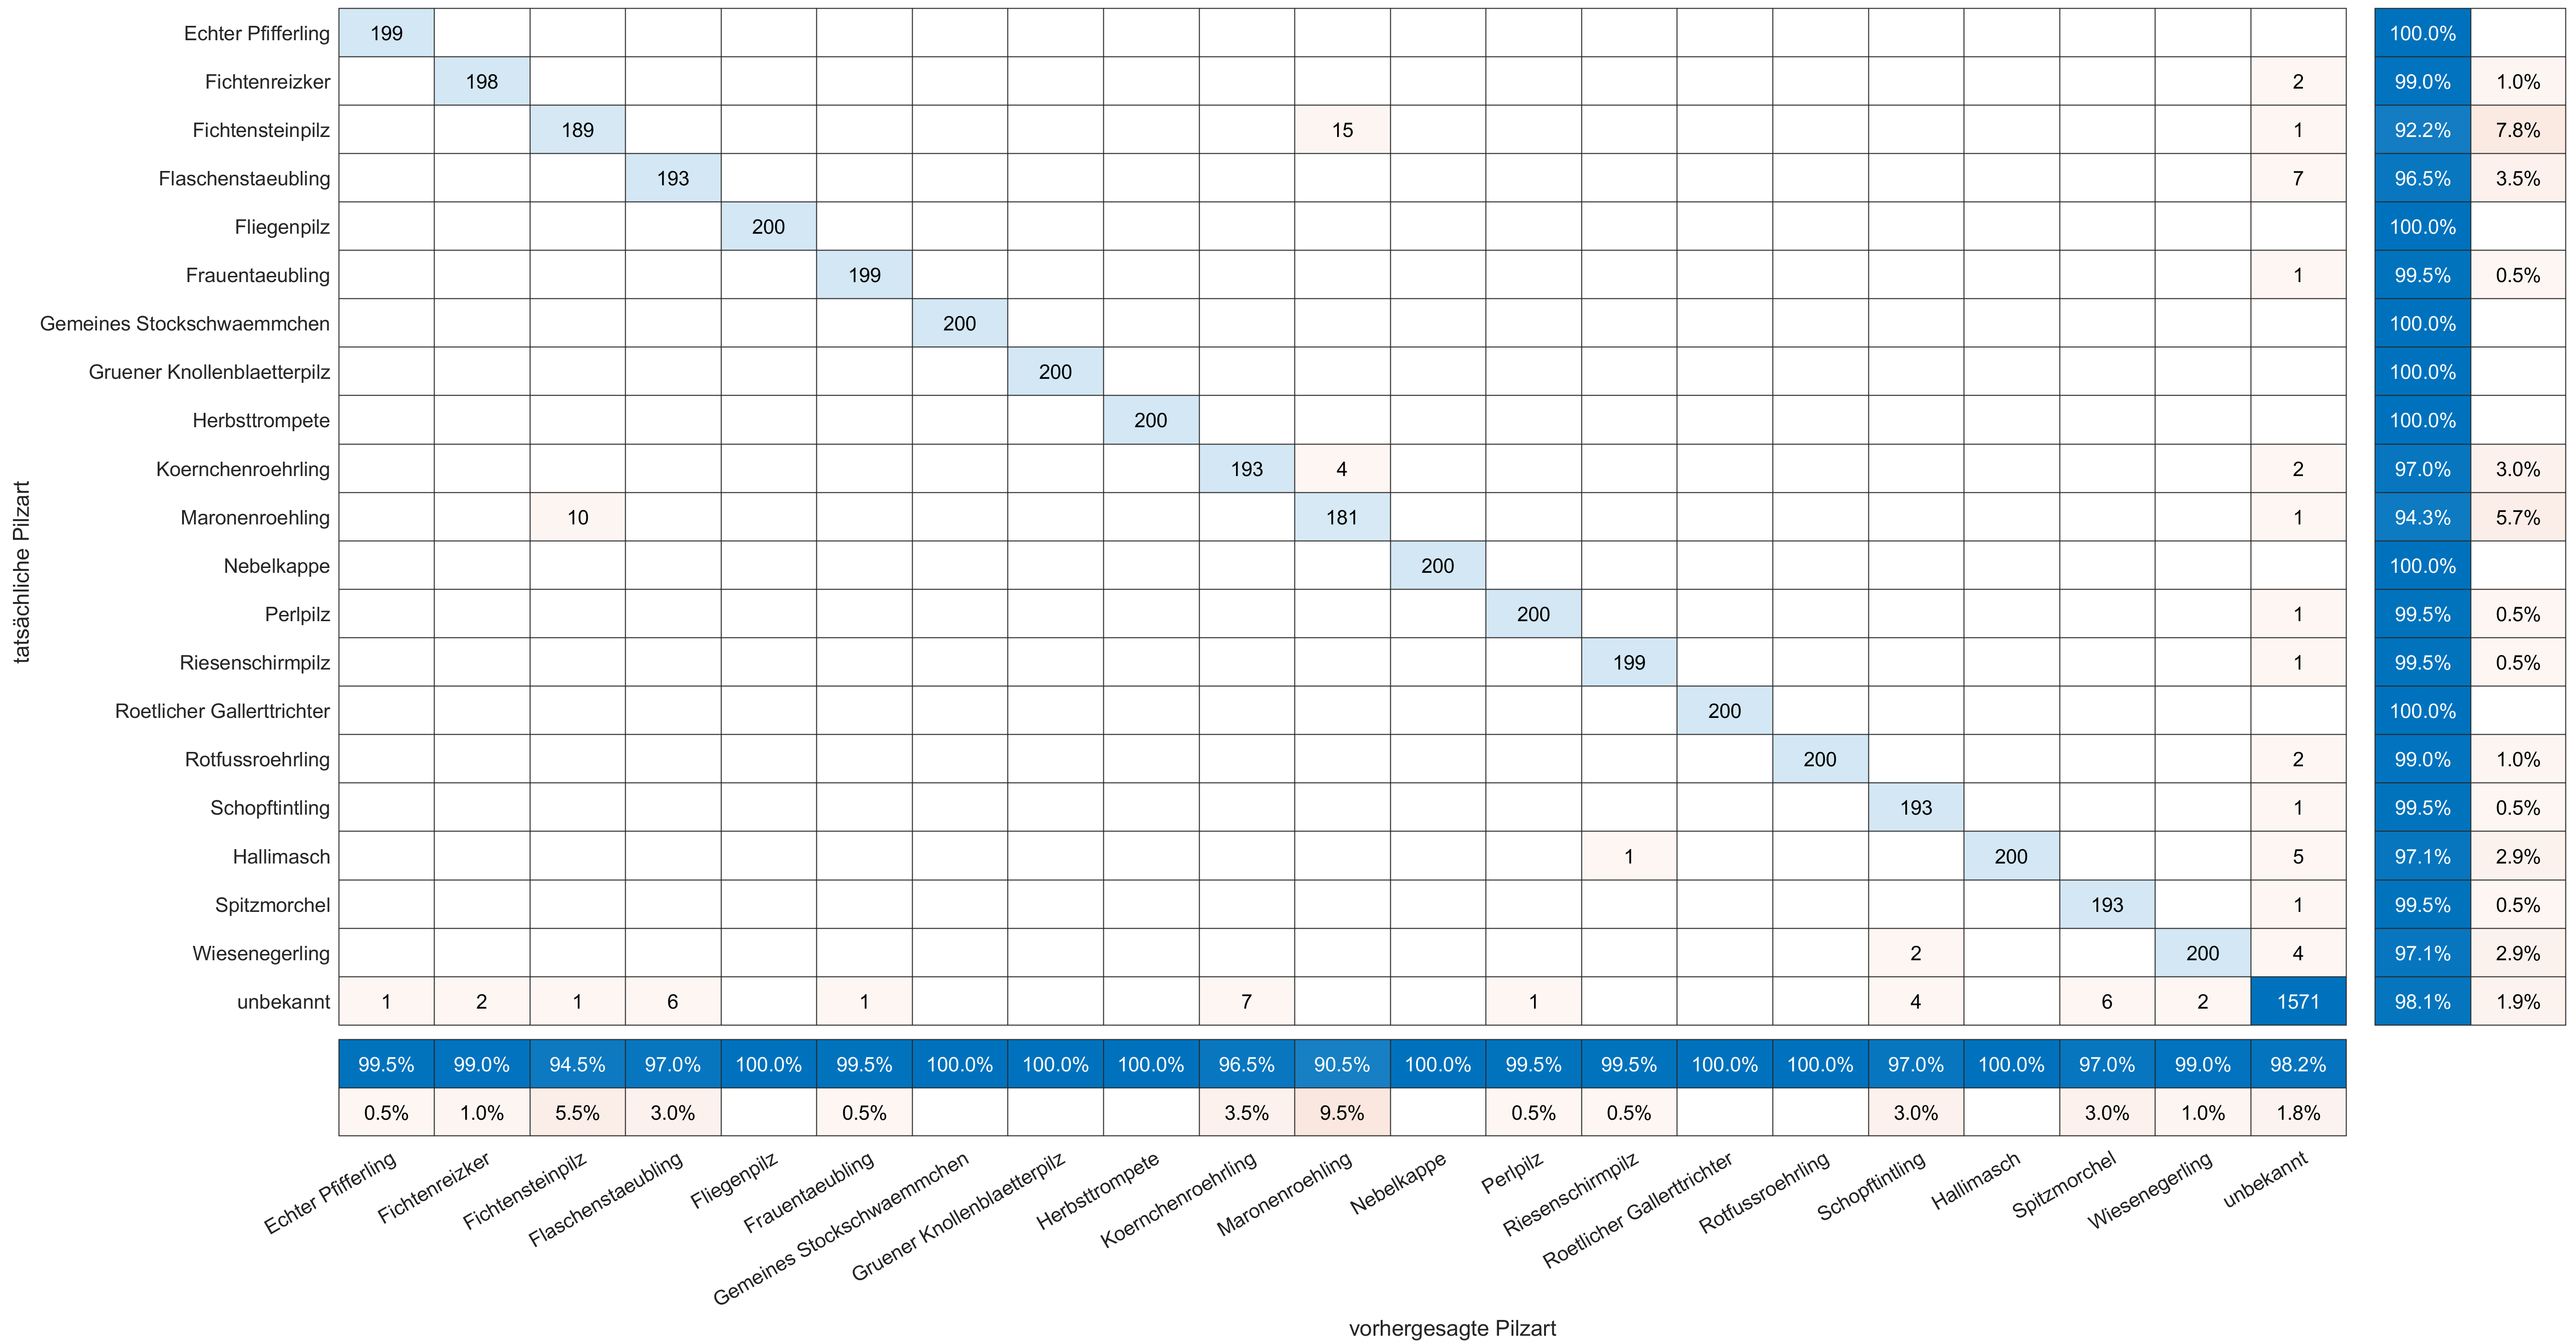
\includegraphics[width=\textwidth]{conf_mat_extra_all}
\caption[Vertauschungsmatrix des Zusatzinformationen-\textit{Transfer-CNN}s mit allen Zusatzinformationen]{Vertauschungsmatrix des Zusatzinformationen-\textit{Transfer-CNN}s, alle Zusatzinformationen für Bestimmung gegeben, Validierungsdaten je zehn mal bestimmt: Auf der Diagonalen befinden sich die Anzahl korrekt klassifizierten Validierungsdaten, die restlichen sind falsch bestimmt worden.}
\label{img:conf_mat_extra_all}
\end{sidewaysfigure}